\underline{\textbf{Issue 1: The first row of the table is empty}}

\begin{table}[h]
\centering
\noindent\adjustbox{max width=\columnwidth}{
\begin{tabular}{|c||c|c|c|c|c|c|c|c|c|c|} % left align
\hline
% remove line in a table, \usepackage{adjustbox}
\multicolumn{10}{|l|}{$V(X) = v_0 + v_1X + v_2X^2 + v_3X^3 + v_4X^4 + v_5X^5 + v_6X^6 + v_7X^7$}  \\ 
\multicolumn{10}{|l|}{\textcolor{white}{......} $ + v_8X^8 + v_9X^9 + v_{10}X^{10} + v_{11}X^{11} + v_{12}X^{12} + v_{13}X^{13} + v_{14}X^{14} + v_{15}X^{15}$}  \\ 
\multicolumn{10}{|l|}{\textcolor{white}{....}$= 0 + 0X +0X^2 +0X^3 +1X^4 +1X^5 +1X^6 +1X^7$}  \\ 
\multicolumn{10}{|l|}{\textcolor{white}{......}$+ 2X^8  + 2X^9 + 2X^{10} + 2X^{11} + 1X^{12} + 1X^{13} + 1X^{14} + 1X^{15}$} \\ 
\hline
\hline
\textbf{\boldmath$i = \hat{\Delta}m + \hat{e}$} & $-8$ & $-7$ & $-6$ & $-5$ & $-4$ & $-3$ & $-2$ & $-1$ \\
(in $V \cdot X^{-i}$) & ($\textcolor{cyan}{}\textcolor{orange}{110}\textcolor{green}{00}_2$) & ($\textcolor{cyan}{}\textcolor{orange}{110}\textcolor{green}{01}_2$) & ($\textcolor{cyan}{}\textcolor{orange}{110}\textcolor{green}{10}_2$) & ($\textcolor{cyan}{}\textcolor{orange}{110}\textcolor{green}{11}_2$) & ($\textcolor{cyan}{}\textcolor{orange}{111}\textcolor{green}{00}_2$) & ($\textcolor{cyan}{}\textcolor{orange}{111}\textcolor{green}{01}_2$) & ($\textcolor{cyan}{}\textcolor{orange}{111}\textcolor{green}{10}_2$) & ($\textcolor{cyan}{}\textcolor{orange}{111}\textcolor{green}{11}_2$)\\
\hline
\textbf{constant term's} & $-2$ & $-2$ & $-2$ & $-2$ & $-1$ & $-1$ & $-1$ & $-1$ \\
 \textbf{coeff. of $V\cdot X^{-i}$}& $\textcolor{orange}{110}_2$ & $\textcolor{orange}{110}_2$ & $\textcolor{orange}{110}_2$ & $\textcolor{orange}{110}_2$ & $\textcolor{orange}{111}_2$ & $\textcolor{orange}{111}_2$ & $\textcolor{orange}{111}_2$ & $\textcolor{orange}{111}\textcolor{green}{00}_2$ \\
\hline
\textbf{$\bm{m}$ (plaintext)} & $-2$ & $-2$ & $-2$ & $-2$ & $-1$ & $-1$ & $-1$ & $-1$ \\
\hline
\hline
\textbf{\boldmath$i = \hat{\Delta}m + \hat{e}$} & $0$ & $1$ & $2$ & $3$ & $4$ & $5$ & $6$ & $7$ \\
(in $V \cdot X^{-i}$) & ($\textcolor{cyan}{}\textcolor{orange}{000}_2$)& ($\textcolor{cyan}{}\textcolor{orange}{000}_2$)& ($\textcolor{cyan}{}\textcolor{orange}{000}_2$)& ($\textcolor{cyan}{}\textcolor{orange}{000}_2$)& ($\textcolor{cyan}{}\textcolor{orange}{001}_2$)& ($\textcolor{cyan}{}\textcolor{orange}{001}_2$)& ($\textcolor{cyan}{}\textcolor{orange}{001}_2$)&($\textcolor{cyan}{}\textcolor{orange}{001}_2$)\\
\hline
\textbf{constant term's} & $0$ & $0$ & $0$ & $0$ & $1$ & $1$ & $1$ & $1$ \\
\textbf{coeff. of $V\cdot X^{-i}$}& $\textcolor{orange}{000}\textcolor{green}{00}_2$ & $\textcolor{orange}{000}\textcolor{green}{00}_2$ & $\textcolor{orange}{000}\textcolor{green}{00}_2$ & $\textcolor{orange}{000}\textcolor{green}{00}_2$ & $\textcolor{orange}{001}\textcolor{green}{00}_2$ & $\textcolor{orange}{001}\textcolor{green}{00}_2$ & $\textcolor{orange}{001}\textcolor{green}{00}_2$ & $\textcolor{orange}{001}\textcolor{green}{00}_2$ \\
\hline
\textbf{$\bm{m}$ (plaintext)} & $0$ & $0$ & $0$ & $0$ & $1$ & $1$ & $1$ & $1$ \\
\hline
\end{tabular}}
\centering
\caption{The Lookup Table for $n=16, q=64, t=8$ LWE setup.
\textcolor{orange}{Orange} is the plaintext $m$'s bits. \textcolor{green}{Green} is the noise $e$'s bits. %\textcolor{cyan}{Cyan} is the 0-padding bit at the MSB of $\hat\Delta m + e$ (and thus the MSB of $m$), ensured by the application's usage of plaintext numbers.
}
\label{tab:lut}
\end{table}






\underline{\textbf{Issue 3: Math error in a table: the empty cell is supposed to have math formulas}}

\begin{table}[h] %usepackage{array} 
\begin{tabular}{|>{\centering\arraybackslash}p{0.1\columnwidth}||>{\centering\arraybackslash}p{0.4\columnwidth}||>{\centering\arraybackslash}p{0.4\columnwidth}|}
\hline \hline
& \textbf{Polynomial over $\bm{X} \bm{\in} \bm{\mathbb{C}}$} & \textbf{Polynomial over $\bm{X} \in \bm{\mathbb{Z}}_{\bm{p}}$} \\ 
& \textbf{(Complex Number)} & \textbf{(Integer Ring)} \\ \hline \hline
\textbf{Definition of the $\bm \mu$-th Root of Unity}& All $X \in \mathbb{C}$ such that $X^\mu = 1$, (which are computed as $X = e^{2 \pi i k / \mu}$ for integer $k$ where $0 \leq k \leq \mu - 1$)& All $X \in \mathbb{Z}_p$ such that $X^\mu \equiv 1 \bmod p$\\ \hline
\textbf{Definition of the Primitive $\bm \mu$-th Root of Unity}& Those $\mu$-th roots of unity $\omega$ such that $\omega^{\mu} = 1$, and $\omega^{\frac{\mu}{2}} \neq 1$ &  Those $\mu$-th roots of unity $\omega$ such that $\omega^{\mu} \equiv 1 \bmod p$, and $\omega^{\frac{\mu}{2}} \not\equiv 1 \bmod p$ \\ \hline
\textbf{Definition of the $\bm \mu$-th Cyclotomic Polynomial} & \multicolumn{2}{|c|}{\shortstack{The polynomial whose roots are the $\mu$-th primitive roots of unity as follows: \\ $ \Phi_{\mu}(x) = \prod_{\omega \in P(\mu)} (x - \omega) $  \text{ } (see Definition~\ref*{subsec:cyclotomic-def} in \autoref{subsec:cyclotomic-def})}}\\ \hline
\textbf{Finding Primitive $\bm \mu$-th Roots of Unity} & For $\omega = e^{2 \pi i/ \mu}$, compute all $\omega^k$ such that $0 < k < \mu $ and $\textsf{gcd}(k, \mu) = 1$  (Theorem~\ref*{subsec:roots-theorem}.4 in \autoref{subsec:roots-theorem}) & Find one satisfactory $\omega$ that is a root of the $\mu$-th cyclotomic polynomial, and compute all $\omega^k \bmod p$ such that $0 < k < \mu $ and $\textsf{gcd}(k, \mu) = 1$ \\ \hline \hline
\end{tabular}
\caption{The roots of unity and cyclotomic polynomials over $X \in \mathbb{C}$ v.s. over $X \in \mathbb{Z}_p$}
\label{tab:cyclotomic-polynomial-comparison}
\end{table}


$ $

\underline{\textbf{Issue 6: sin crashes when used in a caption (see the LaTeX source code that I commented out just below this)}}

%\begin{figure}[h!]
%    \centering
%  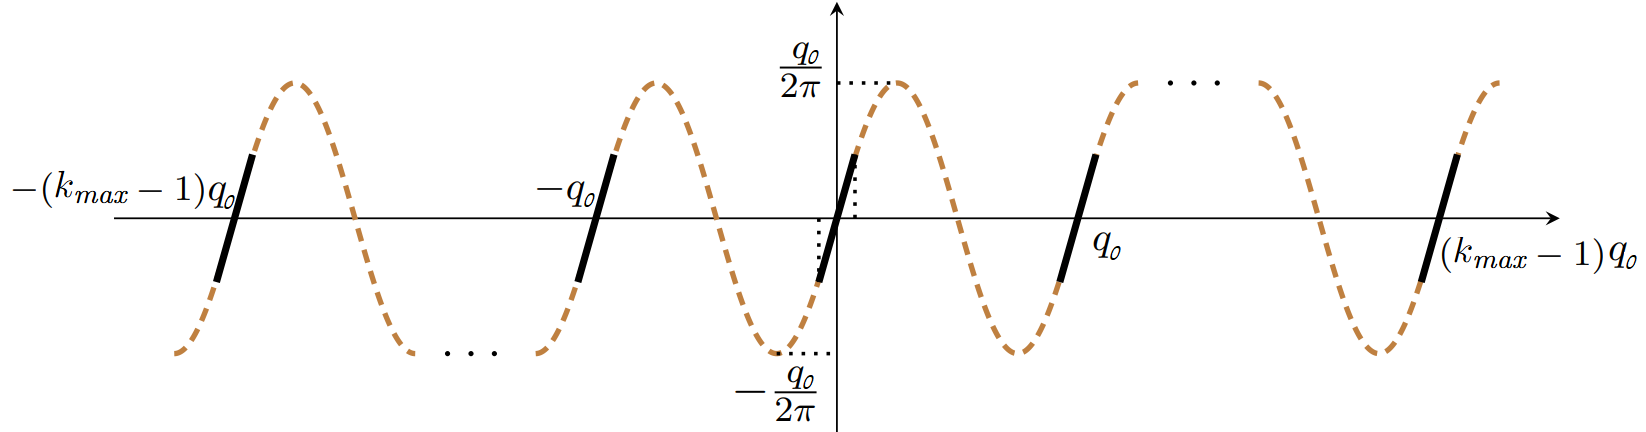
\includegraphics[width=1.0\linewidth]{figures/modulo-reduction-sine.png}
%  \caption{Sine function $f(x) = \dfrac{q_0}{2\pi}\cdot \sin \left(\dfrac{2\pi x}{q_0}\right)$ such that $f(\Delta m_i + e_i + q_0k_i) \approx \Delta m_i + e_i$ (provided $\Delta m_i + e_i \ll q_0$)}
%  \label{fig:modulo-reduction-sine}
%\end{figure}

$ $

\underline{\textbf{Issue 7: Matrix cuts vertically when seeing $\cdots$ twice}}

\noindent $\hathat{W}^* = \begin{bmatrix}
1 & (\omega^{J(0)}) & (\omega^{J(0)})^2 & \cdots & (\omega^{J(0)})^{n-1}\\
1 & (\omega^{J(1)}) & (\omega^{J(1)})^2 & \cdots & (\omega^{J(1)})^{n-1}\\
1 & (\omega^{J(2)}) & (\omega^{J(2)})^2 & \cdots & (\omega^{J(2)})^{n-1}\\
\vdots & \vdots & \vdots & \ddots & \vdots \\
1 & (\omega^{J(\frac{n}{2}-1)}) & (\omega^{J(\frac{n}{2}-1)})^2 & \cdots & (\omega^{J(\frac{n}{2}-1)})^{n-1}\\
1 & (\omega^{J_*(0)}) & (\omega^{J_*(0)})^2 & \cdots & (\omega^{J_*(0)})^{n-1}\\
1 & (\omega^{J_*(1)}) & (\omega^{J_*(1)})^2 & \cdots & (\omega^{J_*(1)})^{n-1}\\
1 & (\omega^{J_*(2)}) & (\omega^{J_*(2)})^2 & \cdots & (\omega^{J_*(2)})^{n-1}\\
\vdots & \vdots & \vdots & \ddots & \vdots \\
1 & (\omega^{J_*(\frac{n}{2}-1)}) & (\omega^{J_*(\frac{n}{2}-1)})^2 & \cdots & (\omega^{J_*(\frac{n}{2}-1)})^{n-1}\\
\end{bmatrix}$

$ $

\underline{\textbf{Issue 11: All citations are broken}}

cite does not work and gives only a question mark. How to make bibliography work? For example, look at this citation: ~\cite{bgv-modswitch1}. 

$ $

\underline{\textbf{Issue 12: Too small vertical gap between each section page's sub-section table and footnote hyperlinks}}

There is an enough space for each part page's table, but there isn't for each section page's table. Could you please add a single space between them? Also, could it be possible to add a title "Section Table" at the top of each section table in a section page? You can refer to the bottom of this page: two last lines. 

$ $

\underline{\textbf{Issue 13: ref* is supposed to remove blue hyperlinks, but it gets preserved, and I cannot possibly remove it... Could you help on this? Click below link and see the blue hyperlink (ref*)}}


\subsection{Polynomial Decomposition}
\label{subsec:poly-decomp}

\begin{tcolorbox}[title={\textbf{\tboxlabel{\ref*{subsec:poly-decomp}} Polynomial Decomposition}}]

Given $f \in \mathbb{Z}_q[z]/(x^n+1)$, where:

$ $

$f = f_1 \dfrac{q}{\beta^1} + f _2\dfrac{q}{\beta^2} + \cdots + f_l \dfrac{q}{\beta^l}  $

$ $

We denote the decomposition of polynomial $f$ into base $\beta$ with level $l$ as follows:

$ $

$\textsf{Decomp}^{\beta, l}(f) = (f_1, f_2, \text{ } \cdots , \text{ } f_l)$
 $ $
\end{tcolorbox}

$ $

\underline{\textbf{Issue 14: Mis-alignment of the title, body, and bullet sections. Could you please make their width the same by choosing the current values of the body section as the default?}}

\title{\Huge{\textbf{The Beginner's Textbook}}\\ \Huge{\textbf{for Fully Homomorphic Encryption}}}

\begin{titlingpage}
\maketitle
\end{titlingpage}

\begin{abstract}
Fully Homomorphic Encryption (FHE) is a cryptographic scheme that enables computations to be performed directly on encrypted data, as if the data were in plaintext. After all computations are performed on the encrypted data, it can be decrypted to reveal the result. The decrypted value matches the result that would have been obtained if the same computations were applied to the plaintext data.

FHE supports basic operations such as addition and multiplication on encrypted numbers. Using these fundamental operations, more complex computations can be constructed, including subtraction, division, logic gates (e.g., AND, OR, XOR, NAND, MUX), and even advanced mathematical functions such as ReLU, sigmoid, and trigonometric functions (e.g., sin, cos). These functions can be implemented either as exact formulas or as approximations, depending on the trade-off between computational efficiency and accuracy. 

Fully Homomorphic Encryption (FHE) enables privacy-preserving machine learning by allowing a server to process the client’s data in its encrypted form through an ML model. With FHE, the server learns neither the plaintext version of the input features nor the inference results. Only the client, using their secret key, can decrypt and access the results at the end of the service protocol.
FHE can also be applied to confidential blockchain services, ensuring that sensitive data in smart contracts remains encrypted and confidential while maintaining the transparency and integrity of the execution process.
Other applications of FHE include secure outsourcing of data analytics, encrypted database queries, privacy-preserving searches, efficient multi-party computation for digital signatures, and more.

This book is designed to help the reader understand how FHE works from the mathematical level. The book comprises the following four parts: 

$ $

\begin{itemize}
\item \textbf{\autoref{part:basic-math}:~\nameref{part:basic-math}} explains necessary background concepts for FHE, such as Group, Field, Order, Polynomial Ring, Cyclotomic Polynomial, Vectors and Matrices, Chinese Remainder Theorem, Taylor Series, Polynomial Interpolation, and Fast Fourier Transform.

\item \textbf{\autoref{part:pqc}:~\nameref{part:pqc}} explains well-known lattice-based cryptographic schemes, which are LWE, RLWE, GLWE, GLev, and GGSW cryptosystems.

\item \textbf{\textbf{\autoref{part:generic-fhe}:~\nameref{part:generic-fhe}}} explains the generic techniques of FHE adopted by many existing schemes, such as homomorphic addition, multiplication, modulus switching, and key switching. 


\item \textbf{\textbf{\autoref{part:fhe-schemes}:~\nameref{part:fhe-schemes}}} explains four widely used FHE schemes: TFHE, BFV, CKKS, and BGV, as well as their RNS-variant versions.
\end{itemize}
\end{abstract}